\documentclass{article}

\usepackage{polski}
\usepackage[utf8]{inputenc}
\usepackage{graphicx}
\graphicspath{ {images/} }

\usepackage{float}
\usepackage{amsmath}
\usepackage{geometry} 

\author{Jakub Postępski}
\title{STP - Projekt I, zadanie 23}
\begin{document}
\maketitle

Obiekt opisany jest transmitancją ciągłą
\[ G(s) = \frac{(s+0.5)(s+3.5)}{(s-6)(s+4)(s+5)} \]
\section{Zadanie 1 - Wyznaczanie modelu w przestrzeni stanów}
Z prostych przekształceń mamy:
\[ G(s) = \frac{s^2 + 4s + 1.75}{s^3 + 3s^2 -34s -120)} = \frac{s^{-1} + 4s^{-2} + 1.75s^{2}}{1 + 3s^{-1} -34s^{-2} -120s^{-3})} = \frac{Y(s)}{U(s)}\]

Przyjmujemy pomocniczy:
\[E(s) = \frac{U(s)}{1 + 3s^{-1} -34s^{-2} -120s^{-3})} = U(s) - 3s^{-1}+34s^{-2} + 120s^{-3}\]
Dodatkowo:
\[Y(s) = (s^{-1} + 4s^{-2} + 1.75s^{2})E(s)\]

Dlatego model (pierwszy wariant metody bezpośredniej, rys. \ref{fig:z11}) w reprezentacji macierzowej:
\[A_1 = \begin{bmatrix} -3 & 34 & 120\\ 1 & 0 & 0\\ 0 & 1 & 0 \end{bmatrix};
B_1 = \begin{bmatrix} 1\\ 0\\ 0 \end{bmatrix};
C_1 = \begin{bmatrix} 1 & 4 & 1.75 \end{bmatrix};
D_1 = 0
\]
\begin{figure}[H]
\centering
\includegraphics[width=0.9\linewidth]{Z1_1}
\caption{Reprezentacja graficzna modelu otrzymanego pierwszym wariantem metody bezpośredniej}
\label{fig:z11}
\end{figure}

Reprezentacje wariantu drugiego metody bezpośredniej (rys. \ref{fig:z12}) otrzymujemy z zależności:
\[A_2 = A_1^T = \begin{bmatrix} -3 & 1 & 0\\ 34 & 0 & 1\\ 120 & 0 & 0 \end{bmatrix};
B_2 = C_1^T = \begin{bmatrix}  1\\ 4\\ 1.75 \end{bmatrix};
C_2 = B_1^T = \begin{bmatrix} 1 & 0 & 0 \end{bmatrix};
D_2 = D_1 = 0
\]
\begin{figure}[H]
\centering
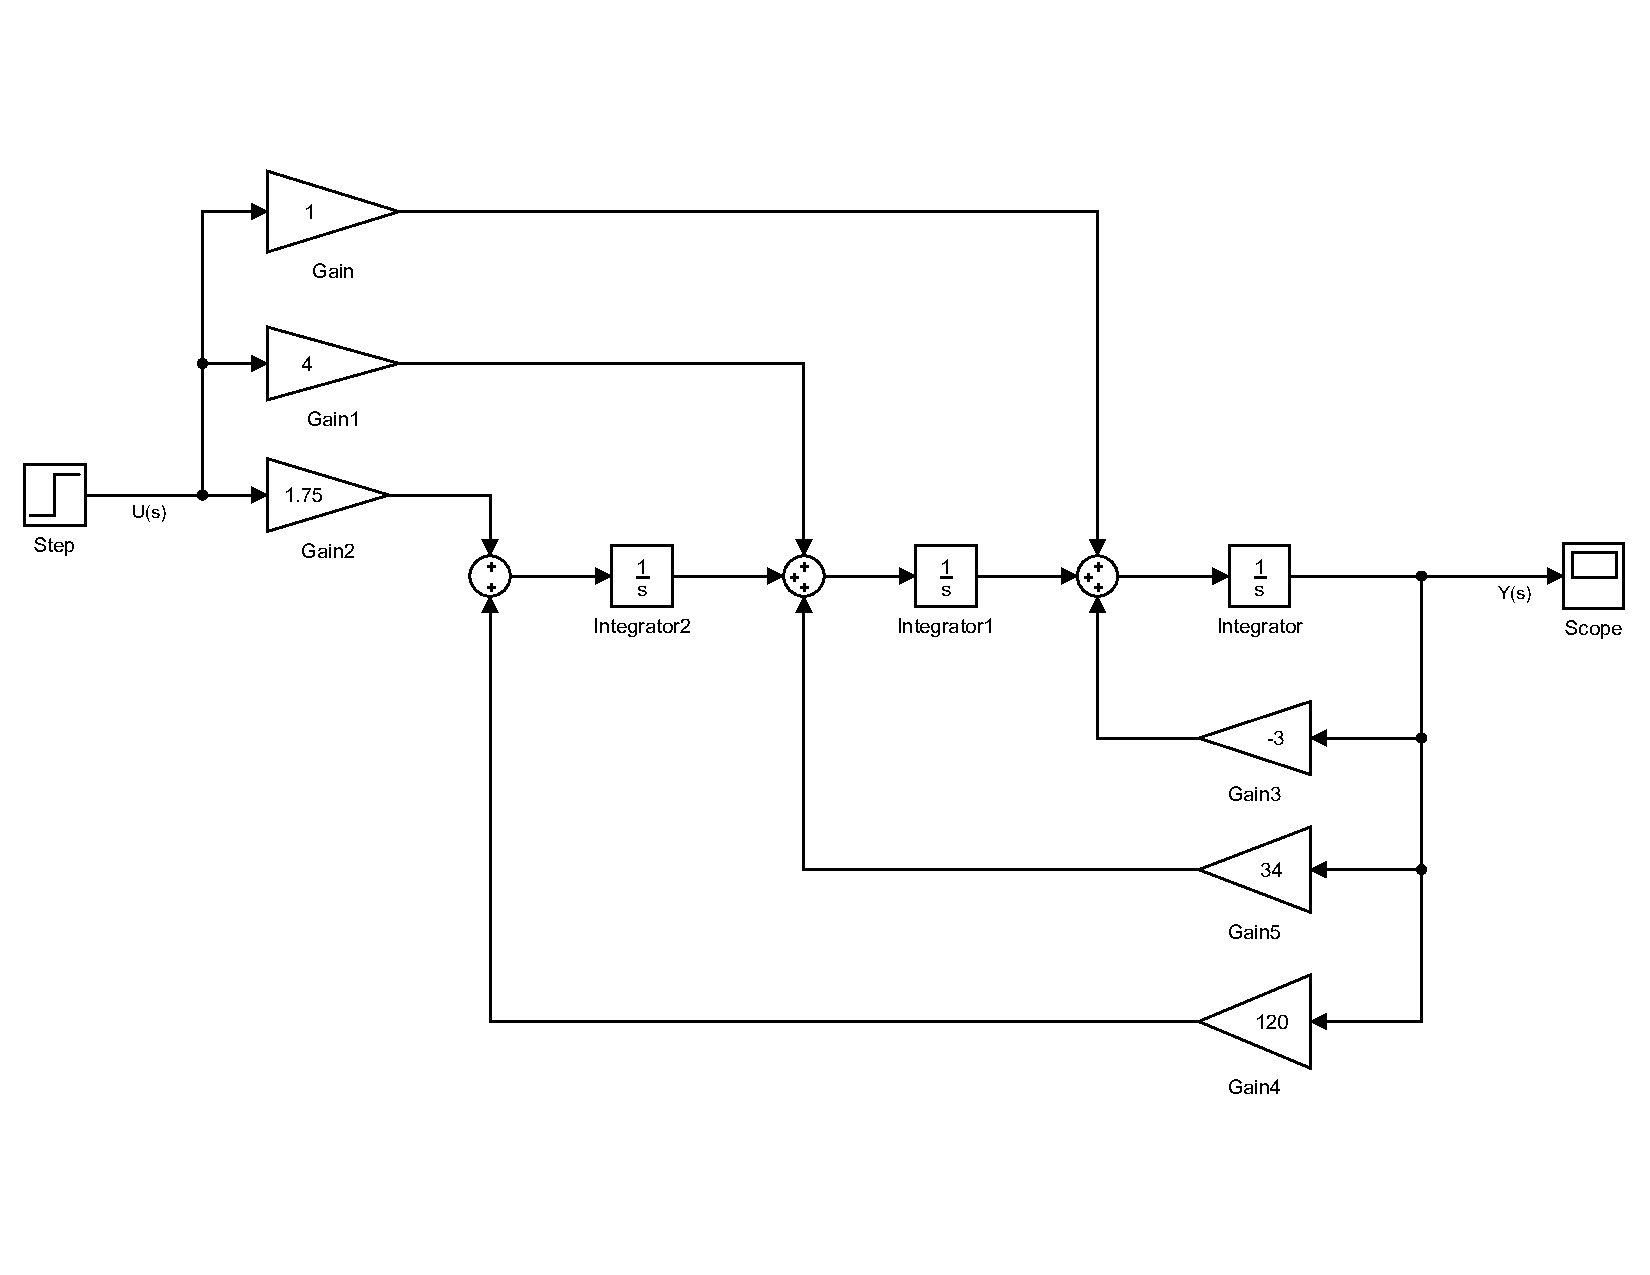
\includegraphics[width=0.9\linewidth]{Z1_2}
\caption{Reprezentacja graficzna modelu otrzymanego drugim wariantem metody bezpośredniej}
\label{fig:z12}
\end{figure}

\section{Zadanie 2 - Dowód, że oba warianty metody bezpośredniej dają tą samą transmitancję}
Dla modelu z pierwszego wariantu metody bezpośredniej mamy macierze postaci:
\[A_1 = \begin{bmatrix} -a_2 & -a_1 & -a_0\\ 1 & 0 & 0\\ 0 & 1 & 0 \end{bmatrix};
B_1 = \begin{bmatrix} 1\\ 0\\ 0 \end{bmatrix};
C_1 = \begin{bmatrix} b_2 & b_1 & b_0 \end{bmatrix};
D_1 = 0
\]

Dla modelu z drugiego wariantu metody bezpośredniej mamy macierze postaci:
\[A_2 = \begin{bmatrix} -a_2 & 1 & 0\\ -a_1 & 0 & 1\\ -a_0 & 0 & 0 \end{bmatrix};
B_2 = \begin{bmatrix}  b_2\\ b_1\\ b_0 \end{bmatrix};
C_2 = \begin{bmatrix} 1 & 0 & 0 \end{bmatrix};
D_2 = 0
\]

Dla wzoru:
\[G(s) = C(sI - A)^{-1}B + D\]

Otrzymujemy:
\[G_1(s) = G_2(s) = \frac{b_2s^{-1} + b_1s^{-2} + b_0s^{2}}{1 + a_2s^{-1} +a_2s^{-2} +a_0s^{-3}}\]
co należało dowieść

\section{Zadanie 3 - Porównanie odpowiedzi skokowej}
Dla $x_0 = \begin{bmatrix}
0 & 0 & 0
\end{bmatrix}$ (rys. \ref{fig:z3})
wszytkie trzy modele jednakowo reagują na odpowiedz skokową. 

\begin{figure}[H]
\centering
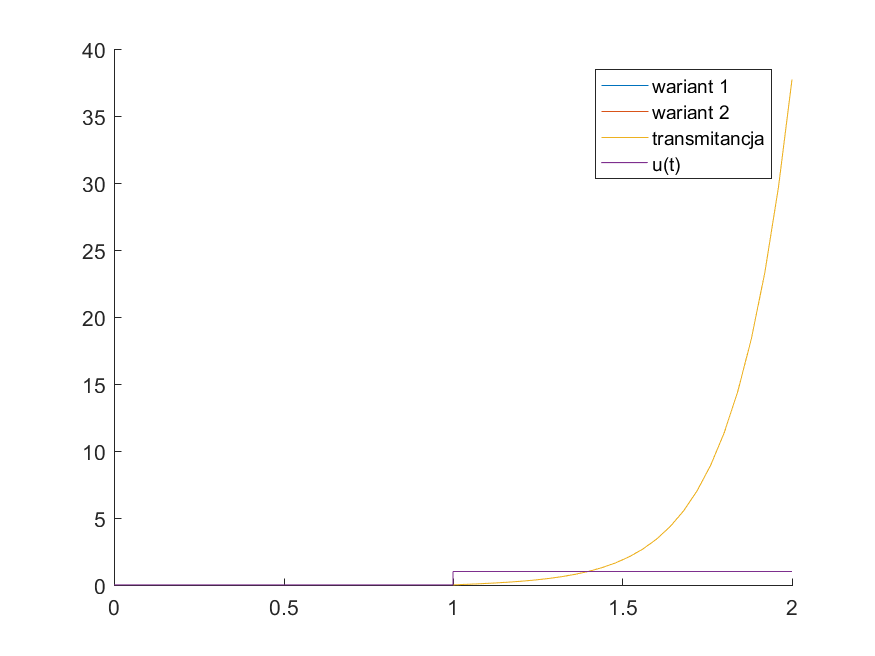
\includegraphics[width=0.9\linewidth]{z3}
\caption{Porównanie odpowiedzi skokowej}
\label{fig:z3}
\end{figure}

Dla $x_0 = \begin{bmatrix}
1 & 1 & 1
\end{bmatrix}$ (rys. \ref{fig:z3a})
Modele są bardziej niestabilne

\begin{figure}[H]
\centering
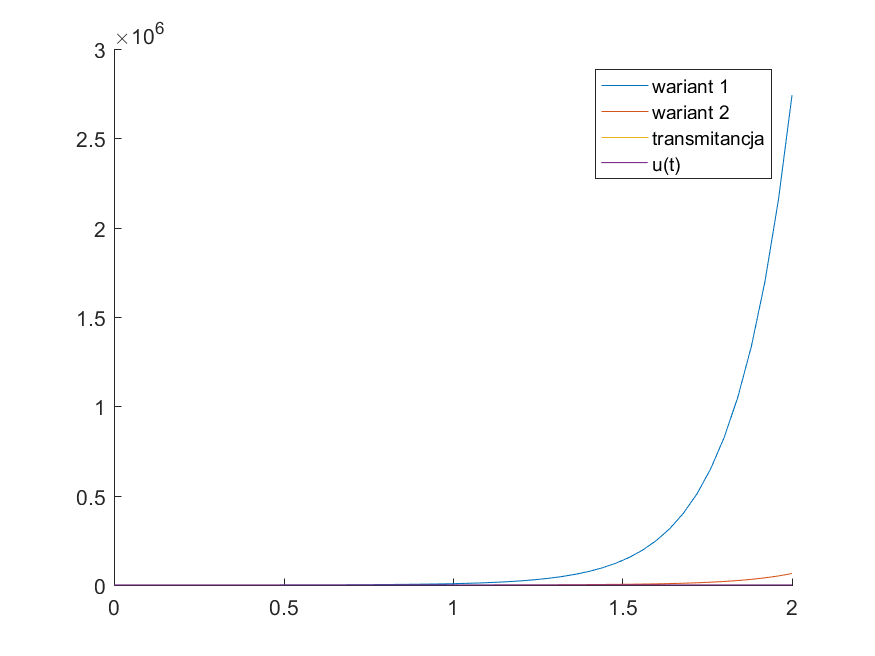
\includegraphics[width=0.9\linewidth]{z3a}
\caption{Porównanie odpowiedzi skokowej}
\label{fig:z3a}
\end{figure}

Dla $x_0 = \begin{bmatrix}
0.1 & 0.1 & 0.1
\end{bmatrix}$ (rys. \ref{fig:z3c}) oraz $x_0 = \begin{bmatrix}
-0.1 & -0.1 & -0.1
\end{bmatrix}$ (rys. \ref{fig:z3b})
Odpowiedzi nie są sysmetryczne względem osi OX.\\
\begin{figure}[H]
\centering
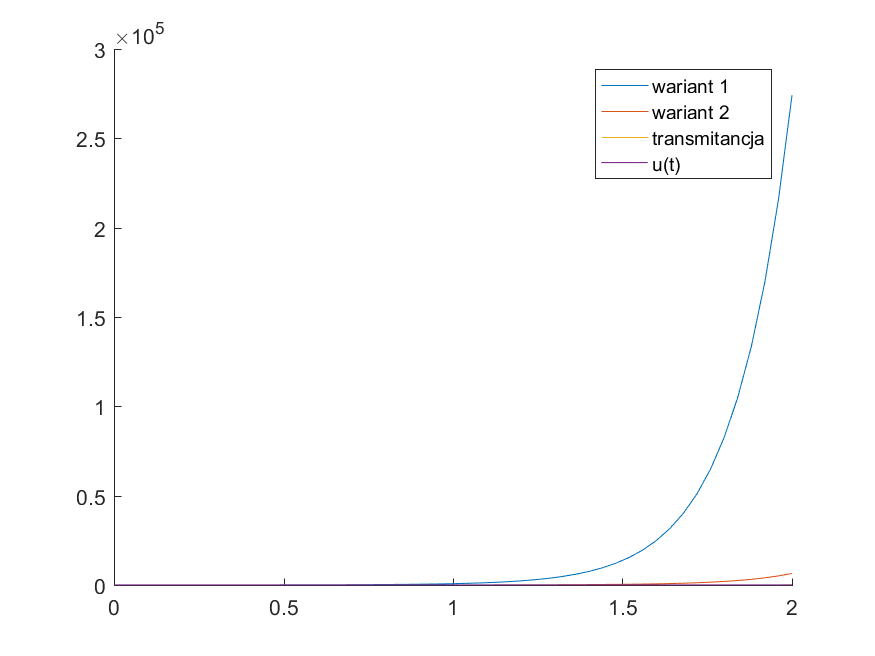
\includegraphics[width=0.9\linewidth]{z3c}
\caption{Porównanie odpowiedzi skokowej}
\label{fig:z3c}
\end{figure}
\begin{figure}[H]
\centering
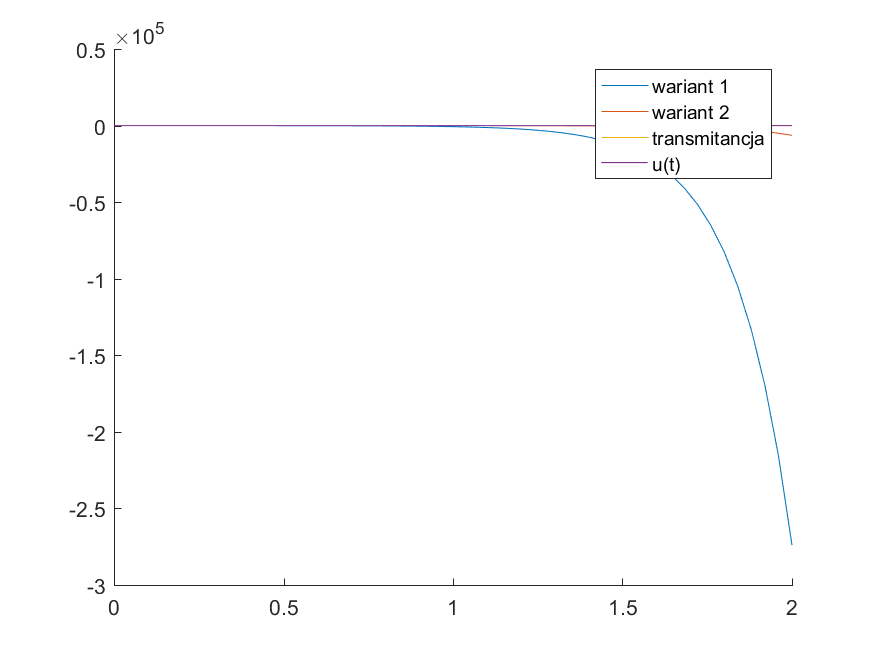
\includegraphics[width=0.9\linewidth]{z3b}
\caption{Porównanie odpowiedzi skokowej}
\label{fig:z3b}
\end{figure}
Jeśli warunki początkowe są takie same, to model będzie reagował na sygnały podobnie. Zmiana warunków początkowych wyraznie zmienia działanie modelu.


\section{Zadanie 5 - Sprawdzenie sterowalności o obserwowalności}
\[det(\begin{bmatrix}B_1 & A_1B_1 & A^2_1B_1\end{bmatrix}) = 
det(\begin{bmatrix} 1 & -3 & 43\\ 0 & 1 & -3\\ 0 & 0 & 1 \end{bmatrix}) = 1 \neq 0\]
Więc obiekt jest sterowalny.

\[det(\begin{bmatrix}C_1 \\ C_1A_1 \\ C_1A^2_1\end{bmatrix}) = 
det(\begin{bmatrix} 1 & 1 & \frac{131}{4}\\ 4 & \frac{143}{4} & 154\\ \frac{7}{4} & 120 & 120 \end{bmatrix}) = -729.4219 \neq 0\]
Więc obiekt jest obserwowalny.

\section{Zadanie 6 - Projektowanie układu regulacji}
Wychodząc od postaci ogólnej regulatora ze sprzężeniem od stanu (rys. \ref{fig:z6_ogolny}) i modyfikując o regulator sprzeżeń od stanu uzyskano układ z rys. \ref{fig:z6}. Dzięki wartościom końcowym postaci $x_{konc} = \begin{bmatrix}
0 & 0 & 0
\end{bmatrix}$ nie było potrzeby stosowania niektórych bloków ze schematu ogólnego. Do obliczania wektora $K$ użyto funkcji \textit{acker()}.

\begin{figure}[H]
\centering
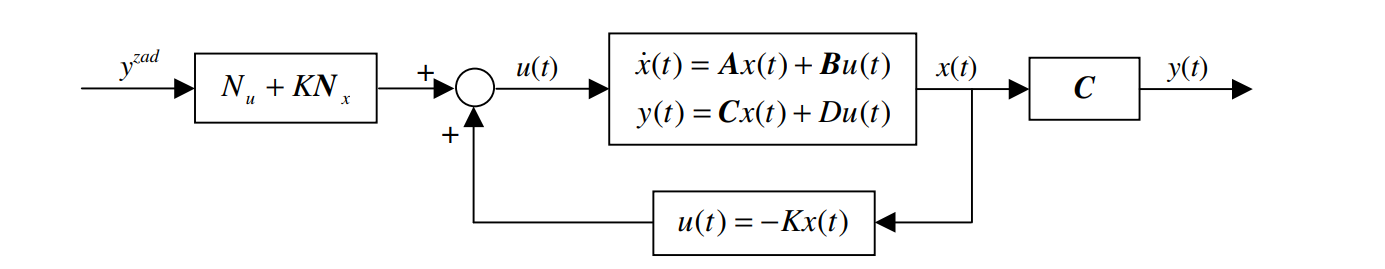
\includegraphics[width=0.9\linewidth]{z6_ogolny}
\caption{Ogólny schemat układu regulacji}
\label{fig:z6_ogolny}
\end{figure}

\begin{figure}[H]
\centering
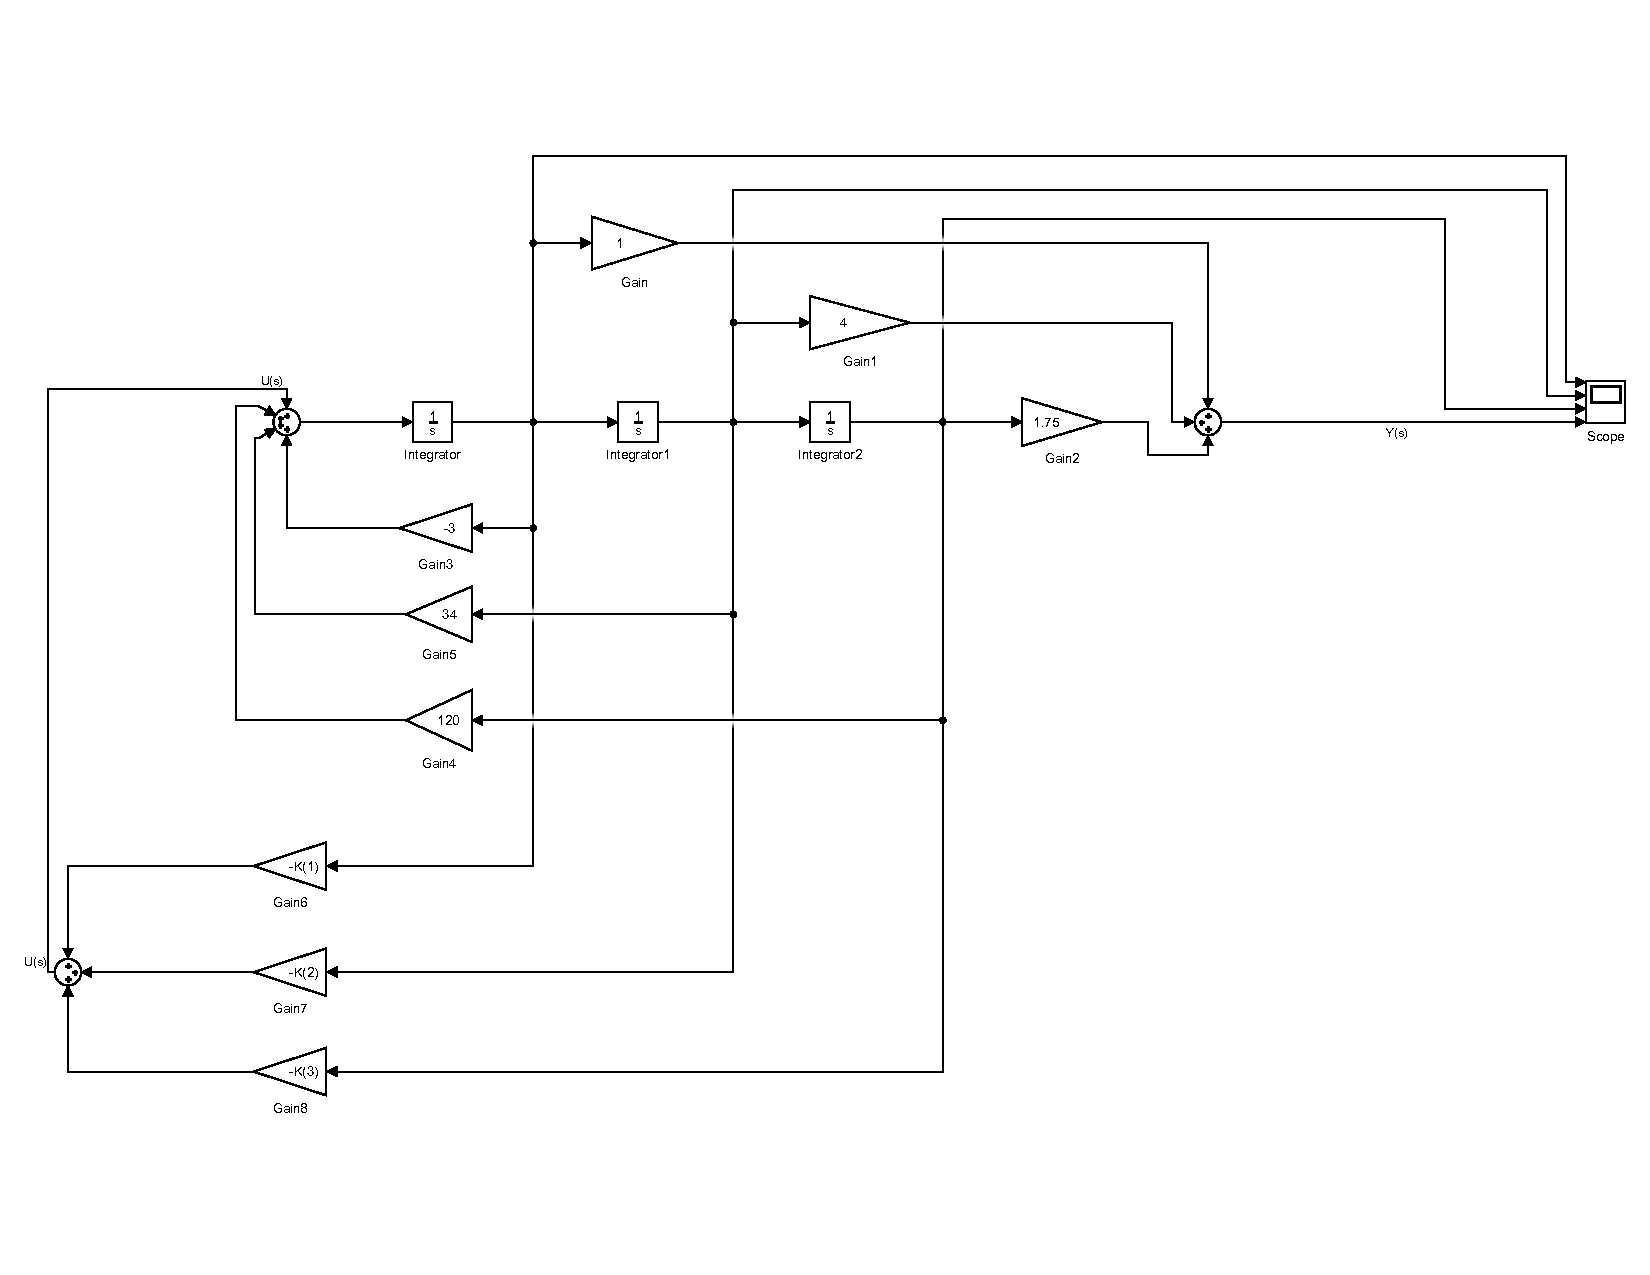
\includegraphics[width=0.9\linewidth]{z6}
\caption{Model z podłączonym układem regulacji}
\label{fig:z6}
\end{figure}

Przyjmując $x_{pocz} = \begin{bmatrix}-1 & 2 & 1\end{bmatrix}^T$ testowano układy przyjmując:
\begin{itemize}
\item trzy jednakowe rzeczywiste bieguny (rys. \ref{fig:z6-4}, rys. \ref{fig:z6-2}, rys. \ref{fig:z6-01}, rys. \ref{fig:z60}, rys. \ref{fig:z61})
\item jeden biegun rzeczywisty $s_1 = -1$ i dwa sprzężone postaci $s_2, s_3 = a \pm ib$ (rys. \ref{fig:z6-11}, \ref{fig:z6-1-1}, \ref{fig:z6-41}, \ref{fig:z6-201}, \ref{fig:z6-21}, \ref{fig:z611})
\end{itemize}

\begin{figure}[H]
\centering
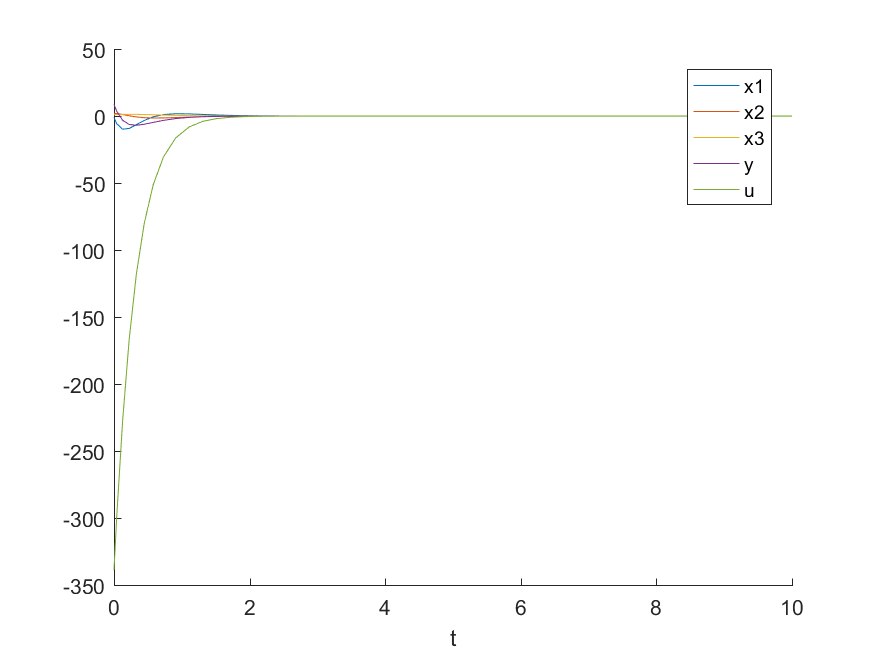
\includegraphics[width=0.9\linewidth]{z6_-4}
\caption{Bieguny regulacji: $s_1 = s_2 = s_3 = -4$. Układ stabilny. Duża zmiana i amplituda sygnału wejściowego. Szybka regulacja.}
\label{fig:z6-4}
\end{figure}

\begin{figure}[H]
\centering
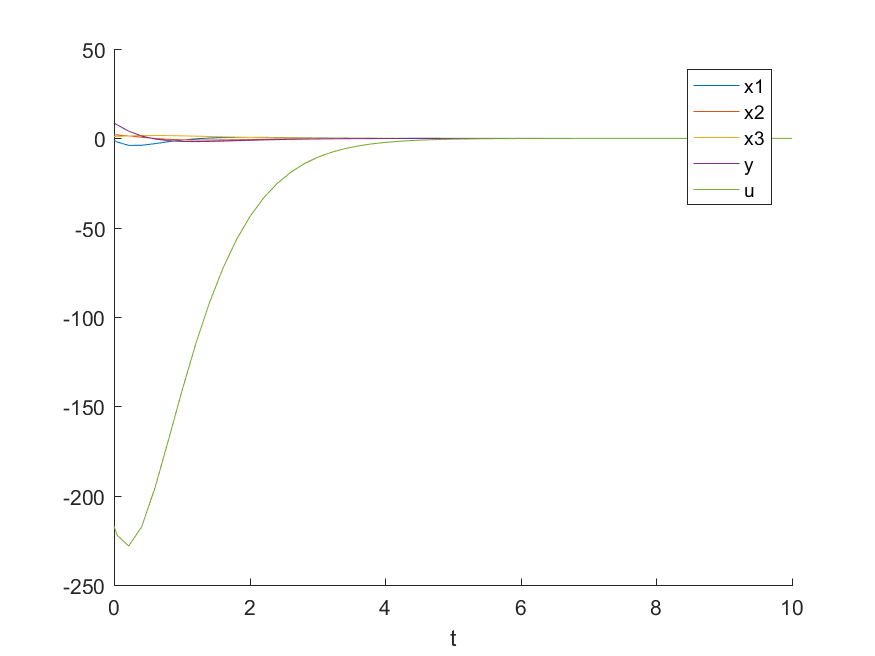
\includegraphics[width=0.9\linewidth]{z6_-2}
\caption{Bieguny regulacji: $s_1 = s_2 = s_3 = -2$. Układ stabilny. Optymalna zmiana i amplituda sygnału wejściowego.}
\label{fig:z6-2}
\end{figure}

\begin{figure}[H]
\centering
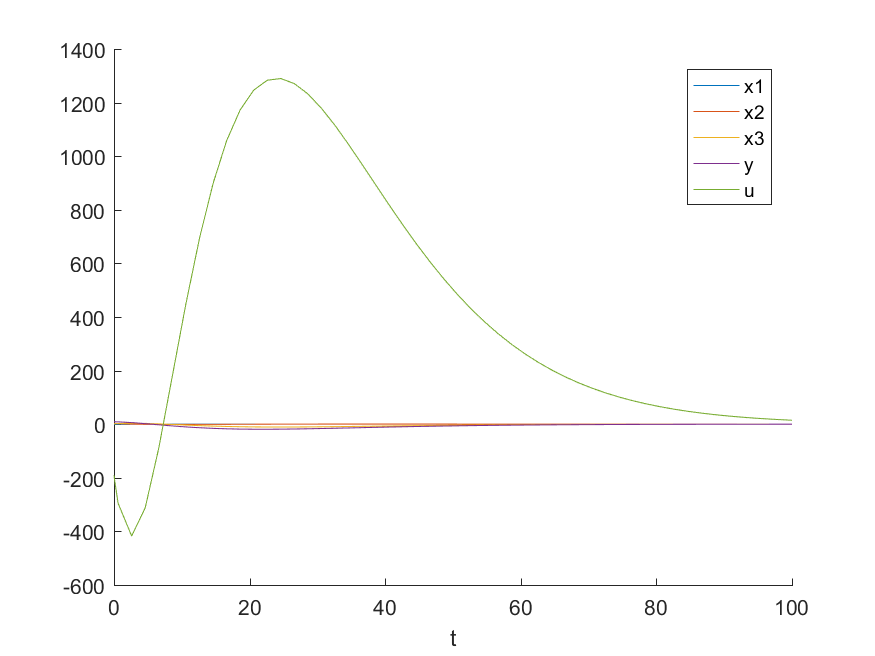
\includegraphics[width=0.9\linewidth]{z6_-01}
\caption{Bieguny regulacji: $s_1 = s_2 = s_3 = 0$. Układ stabilny. Przeregulowanie. Wolna regulacja.}
\label{fig:z6-01}
\end{figure}


\begin{figure}[H]
\centering
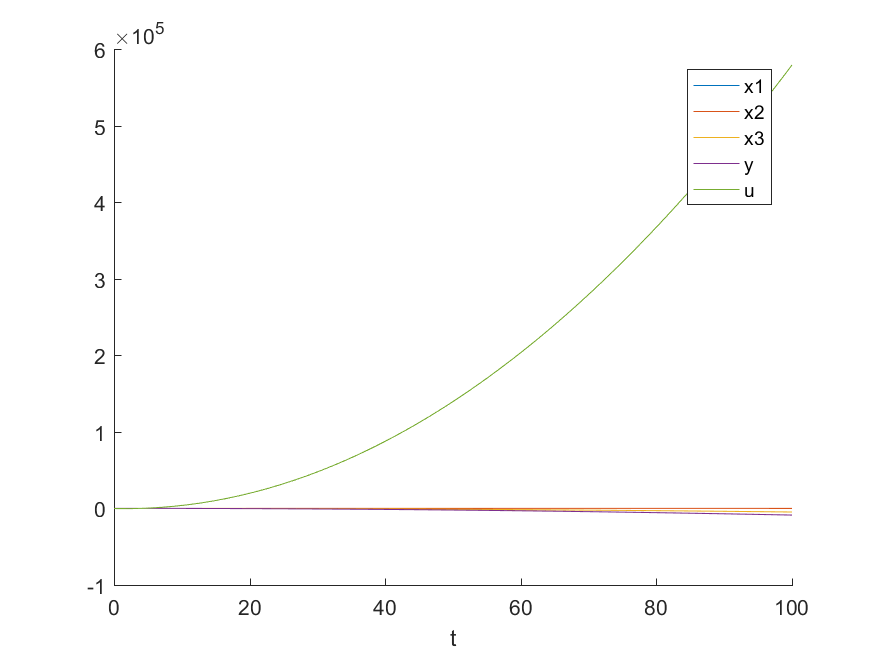
\includegraphics[width=0.9\linewidth]{z6_0}
\caption{Bieguny regulacji: $s_1 = s_2 = s_3 = 0$. Układ niestabilny.}
\label{fig:z60}
\end{figure}

\begin{figure}[H]
\centering
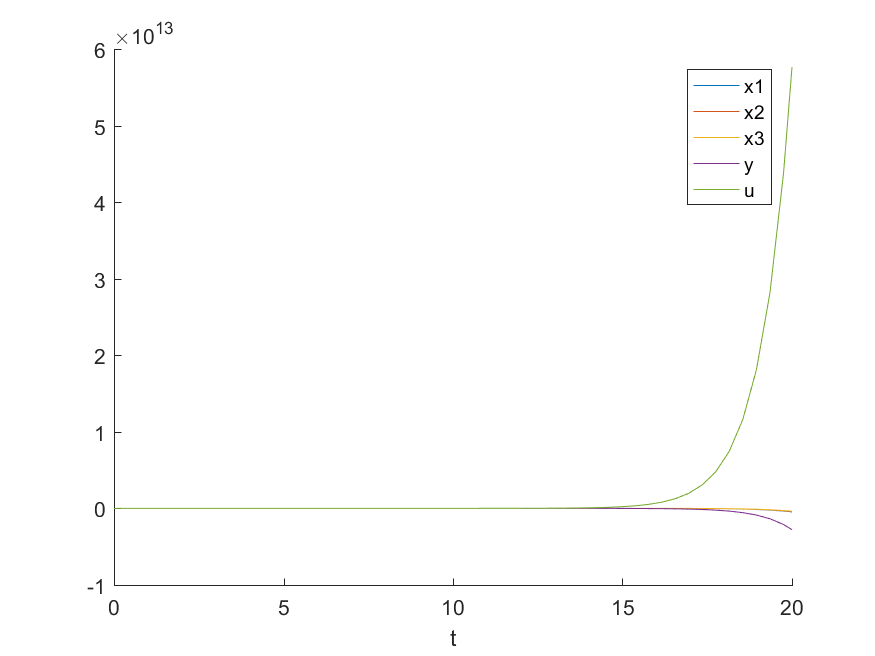
\includegraphics[width=0.9\linewidth]{z6_1}
\caption{Bieguny regulacji: $s_1 = s_2 = s_3 = 1$. Układ niestabilny.}
\label{fig:z61}
\end{figure}



\begin{figure}[H]
\centering
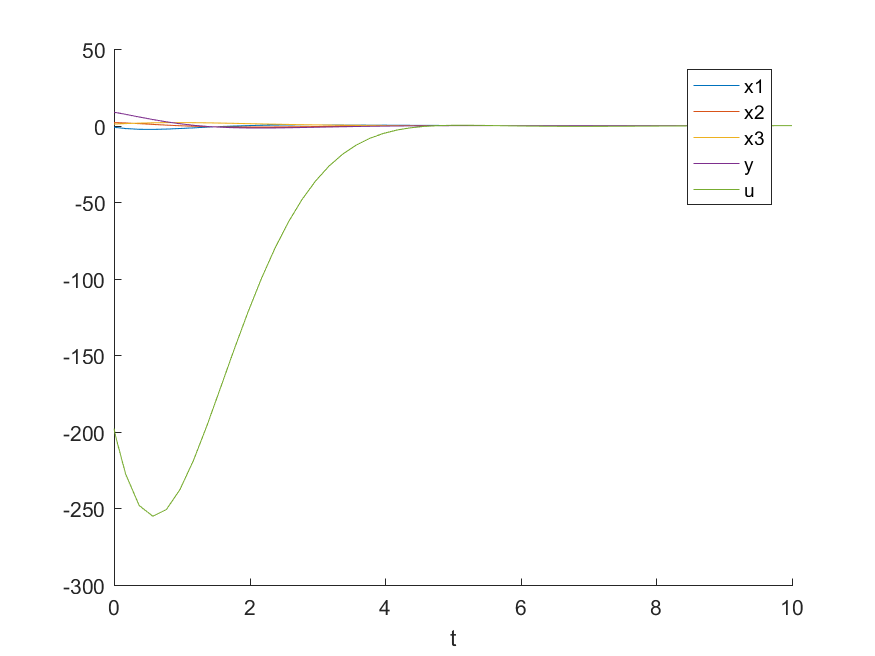
\includegraphics[width=0.9\linewidth]{z6_-1,1}
\caption{Bieguny regulacji: $a = -1 b = 1$. Układ stabilny.}
\label{fig:z6-11}
\end{figure}

\begin{figure}[H]
\centering
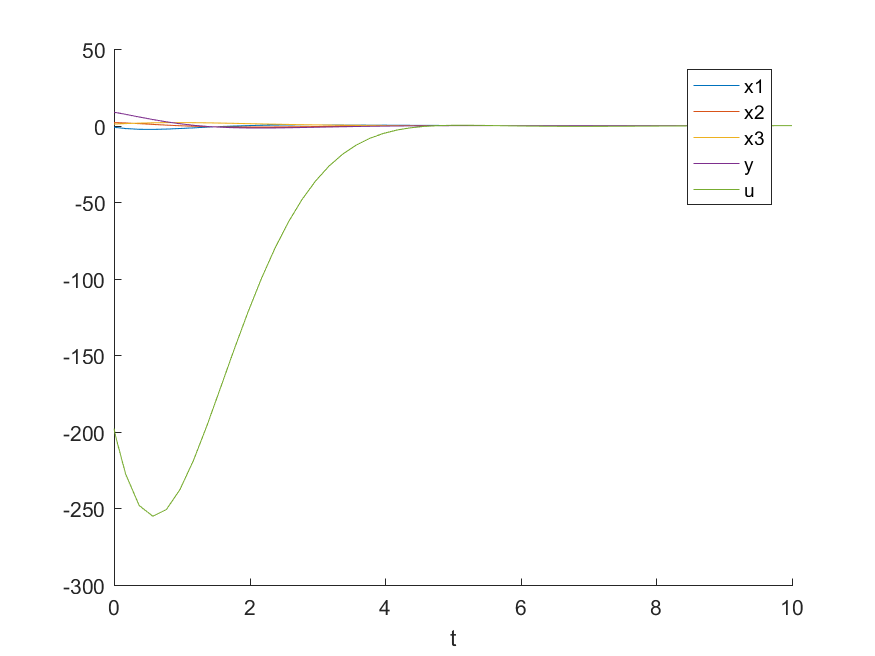
\includegraphics[width=0.9\linewidth]{z6_-1,-1}
\caption{Bieguny regulacji: $a = -1 b = -1$. Układ stabilny. Brak różnic w sygnale wejściowym i wyjściowym modelu w stosunku do rys. \ref{fig:z6-11}}
\label{fig:z6-1-1}
\end{figure}

\begin{figure}[H]
\centering
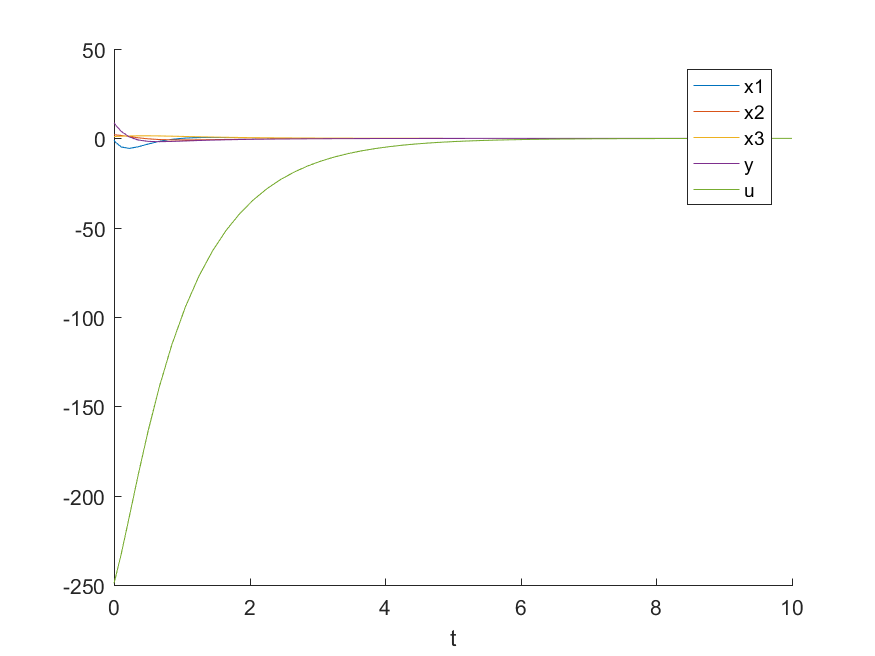
\includegraphics[width=0.9\linewidth]{z6_-4,1}
\caption{Bieguny regulacji: $a = -4 b = 1$. Układ stabilny.}
\label{fig:z6-41}
\end{figure}

\begin{figure}[H]
\centering
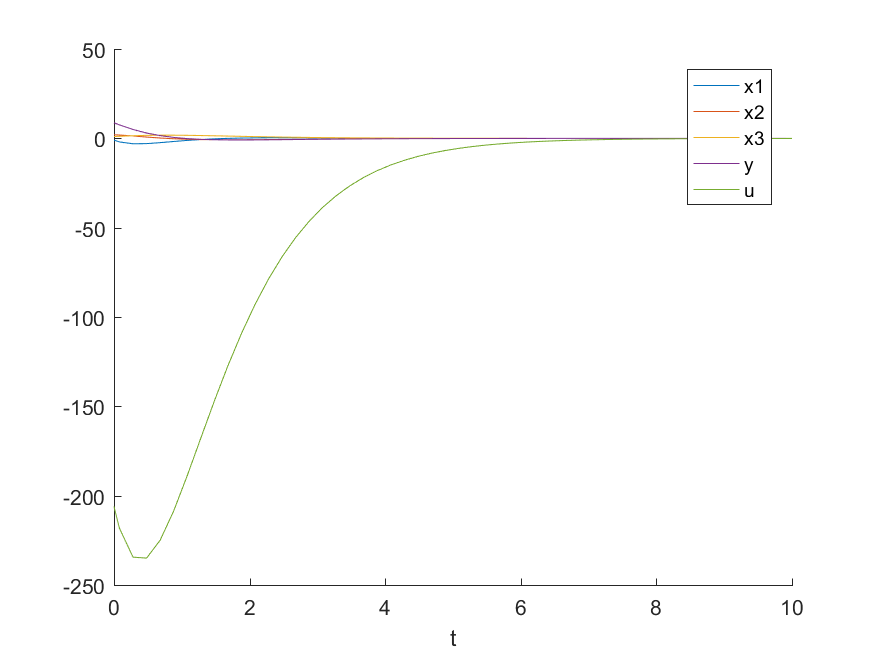
\includegraphics[width=0.9\linewidth]{z6_-2,01}
\caption{Bieguny regulacji: $a = -2 b = 0.1$. Układ stabilny. Zmiana sygnału sterującego i czas regulacji optymalny.}
\label{fig:z6-201}
\end{figure}

\begin{figure}[H]
\centering
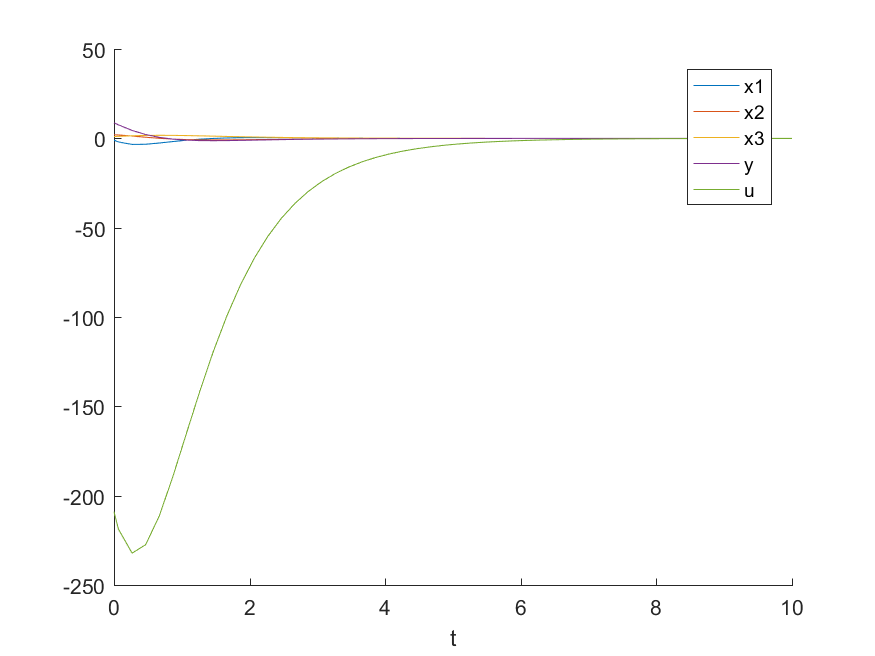
\includegraphics[width=0.9\linewidth]{z6_-2,-1}
\caption{Bieguny regulacji: $a = -2 b = -1$. Układ stabilny.}
\label{fig:z6-21}
\end{figure}

\begin{figure}[H]
\centering
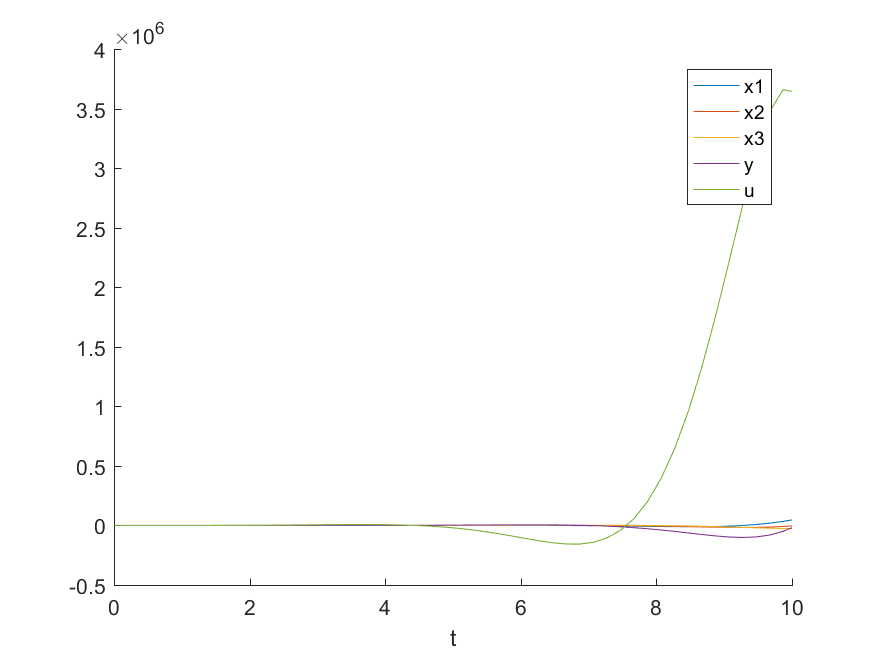
\includegraphics[width=0.9\linewidth]{z6_1,1}
\caption{Bieguny regulacji: $a = 1 b = 1$. Układ niestabilny.}
\label{fig:z611}
\end{figure}

Wnioski ogólne:
\begin{itemize}
\item Układ jest stabilny tylko jeśli bieguny znajdują się w prawej półpłaszczyznie.
\item Im bardziej bieguny przesunięte są w stronę liczb ujemnych tym szybciej następuje regulacja. Odbywa się to kosztem zwiększenia zmian sygnału sterującego.
\item Układ z biegunami ujemnymi bliskimi zera reguluje się wolniej.
\item W przypadku badanego modelu najlepiej zadziałał regulator z biegunami $s_1 = s_2 = s_3 = -2$.
\end{itemize}
\section{Zadanie 7 - Sterowanie wartością zadaną}
Przyjęto układ regulacji z rys. \ref{fig:z6_ogolny}. \\
Z zależności:
\[ \begin{bmatrix} N_x \\ N_u \end{bmatrix}
= \begin{bmatrix} A_1 & B_1 \\ C_1 & D_1 \end{bmatrix}^{-1}\begin{bmatrix}0\\0\\0\\1 \end{bmatrix}\]
wyliczono:
\[N_x = \begin{bmatrix}0 \\ 0\\0.5714\end{bmatrix}\]
\[N_u = \begin{bmatrix}-68.5714\end{bmatrix}\]

Przetestowano układ z wartością zadaną (rys. \ref{fig:z71} oraz \ref{fig:z72}). Cały układ wraz z regulatorem przedstawia rys. \ref{fig:z7}.

\begin{figure}[H]
\centering
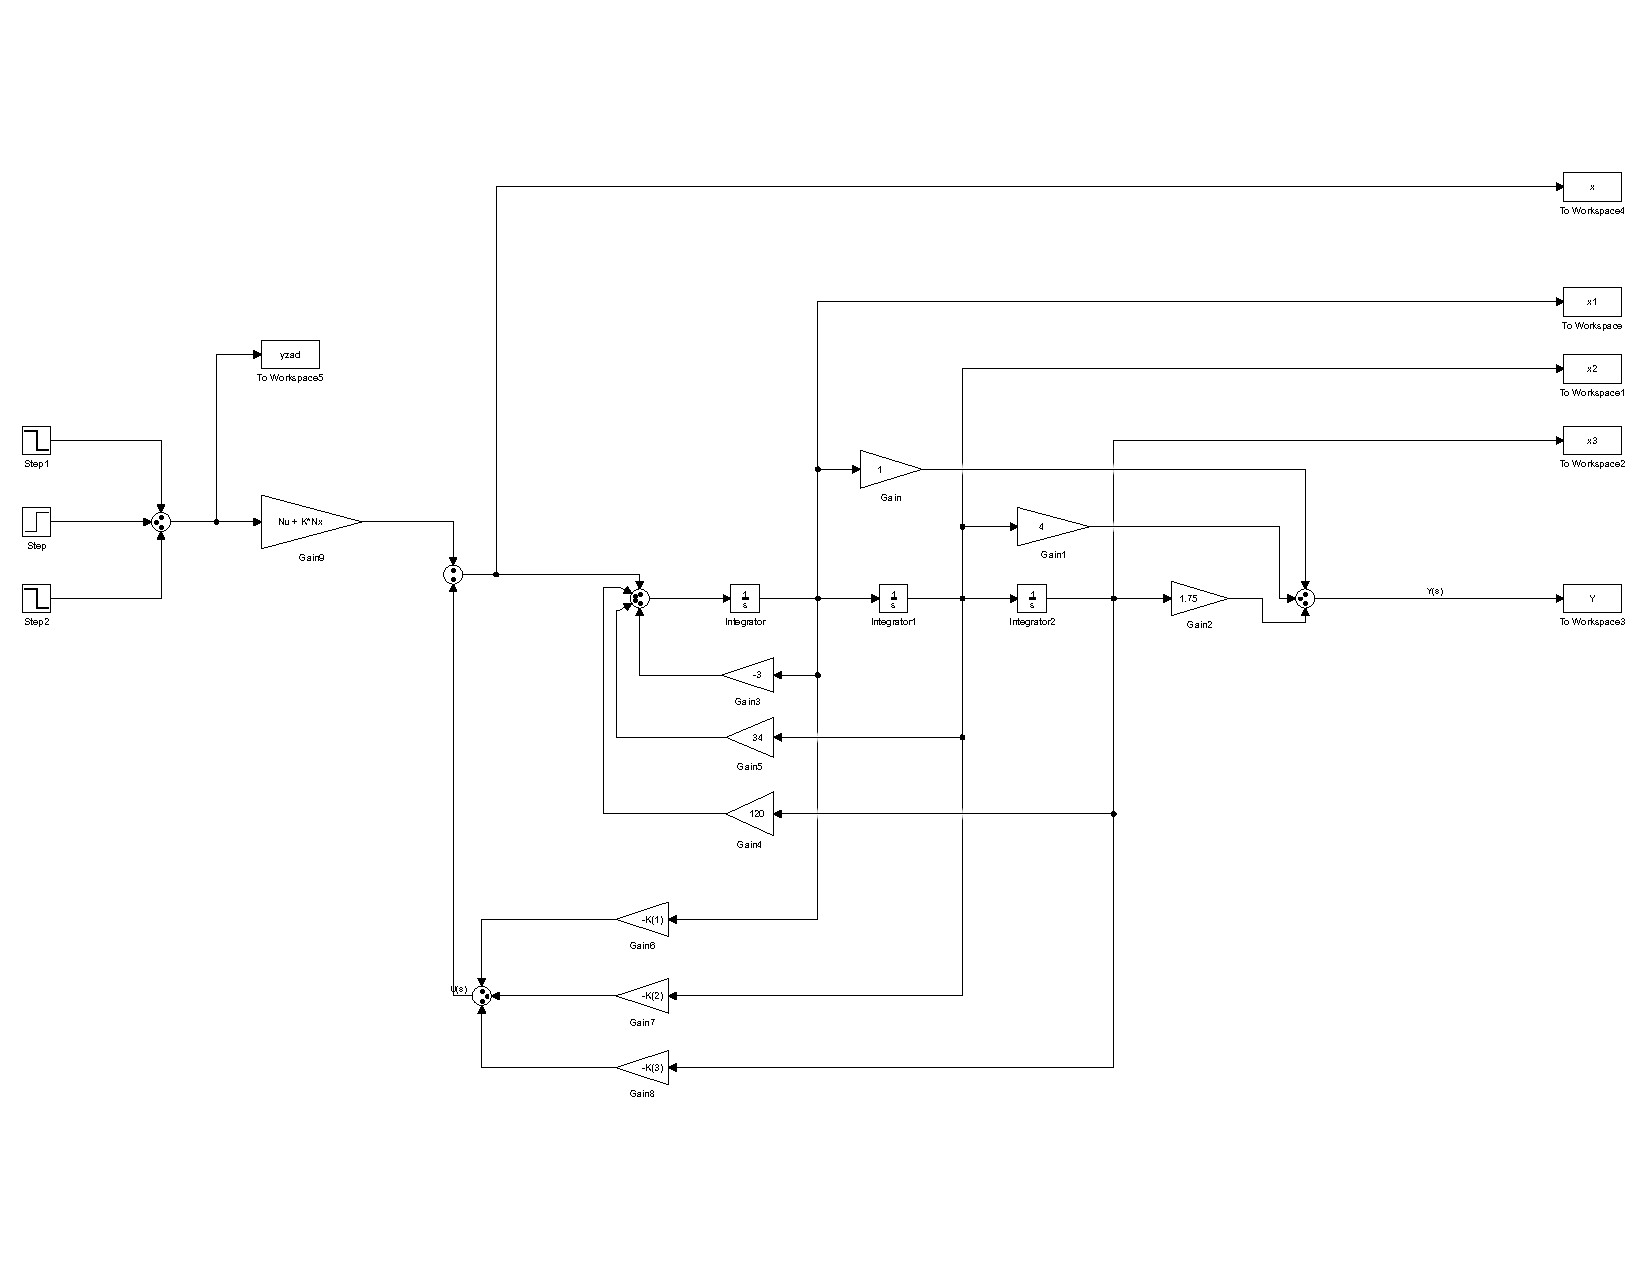
\includegraphics[width=0.9\linewidth]{z7}
\caption{Struktura układu z regulatorem.}
\label{fig:z7}
\end{figure}


\begin{figure}[H]
\centering
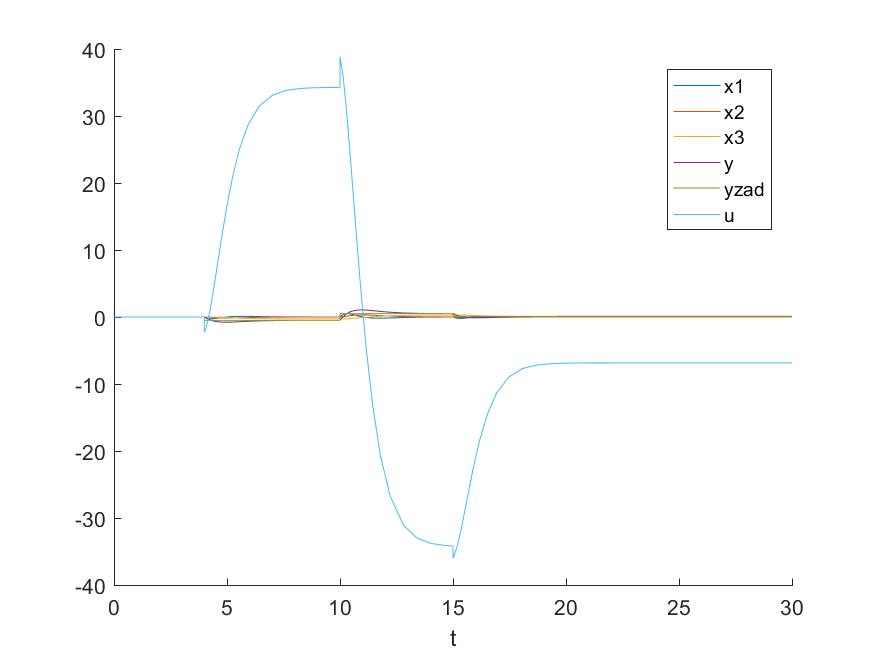
\includegraphics[width=0.9\linewidth]{z71}
\caption{Bieguny regulacji: $s_1 = s_2 = s_3 = -2$. Układ nadąża za zmianami sygnału sterującego.}
\label{fig:z71}
\end{figure}

\begin{figure}[H]
\centering
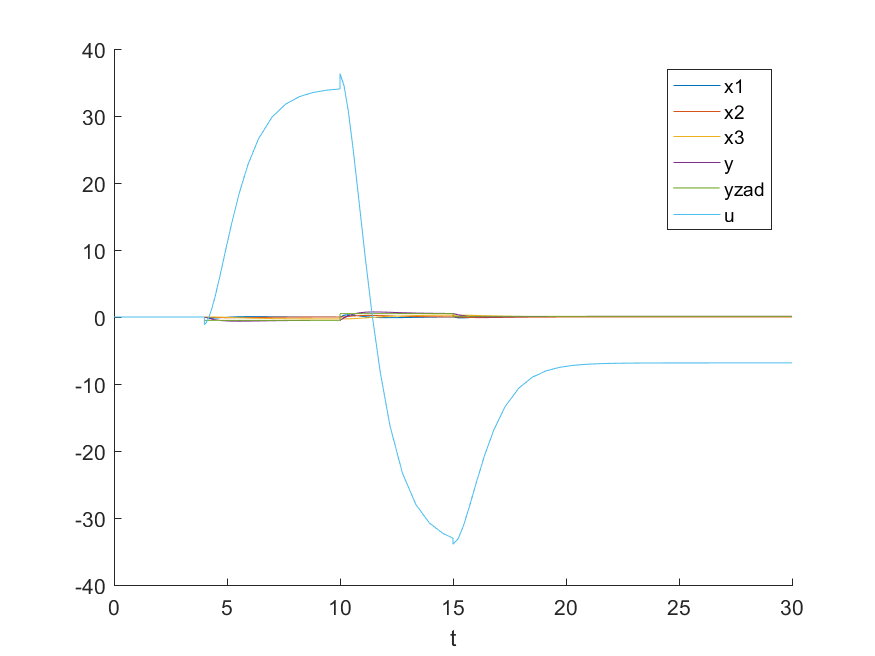
\includegraphics[width=0.9\linewidth]{z72}
\caption{Bieguny regulacji: $s_1 = -1; s_2 = -2 + 0.1i; s_3 = -2 -0.1i$. Układ reguluje się nieznacznie szybciej.}
\label{fig:z72}
\end{figure}
\section{Zadanie 8 - Obserwator pełnego rzędu}
Układ z obserwatorem(rys. \ref{fig:z8osb}) opisuje równanie:
\[\dot{\hat{x}} = A\hat{x}(t) + Bu(t) + L(y(t)-C\hat{x}(t))\]
Układ układu z regulatorem i obserwatorem przedstawia rys. \ref{fig:z8reg}. Zrealizowano układ (rys. \ref{fig:z8sim})

\begin{figure}[H]
\centering
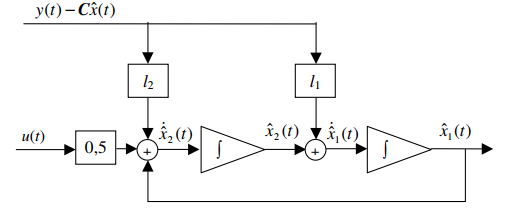
\includegraphics[width=0.9\linewidth]{z8obs}
\caption{Ogólna struktura obserwatora}
\label{fig:z8osb}
\end{figure}

\begin{figure}[H]
\centering
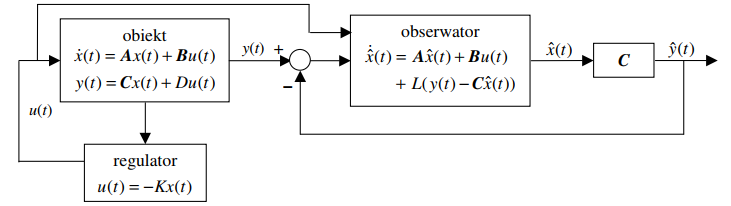
\includegraphics[width=0.9\linewidth]{z8reg}
\caption{Ogólna struktura układu z obserwatorem i regulatorem}
\label{fig:z8reg}
\end{figure}

\begin{figure}[H]
\centering
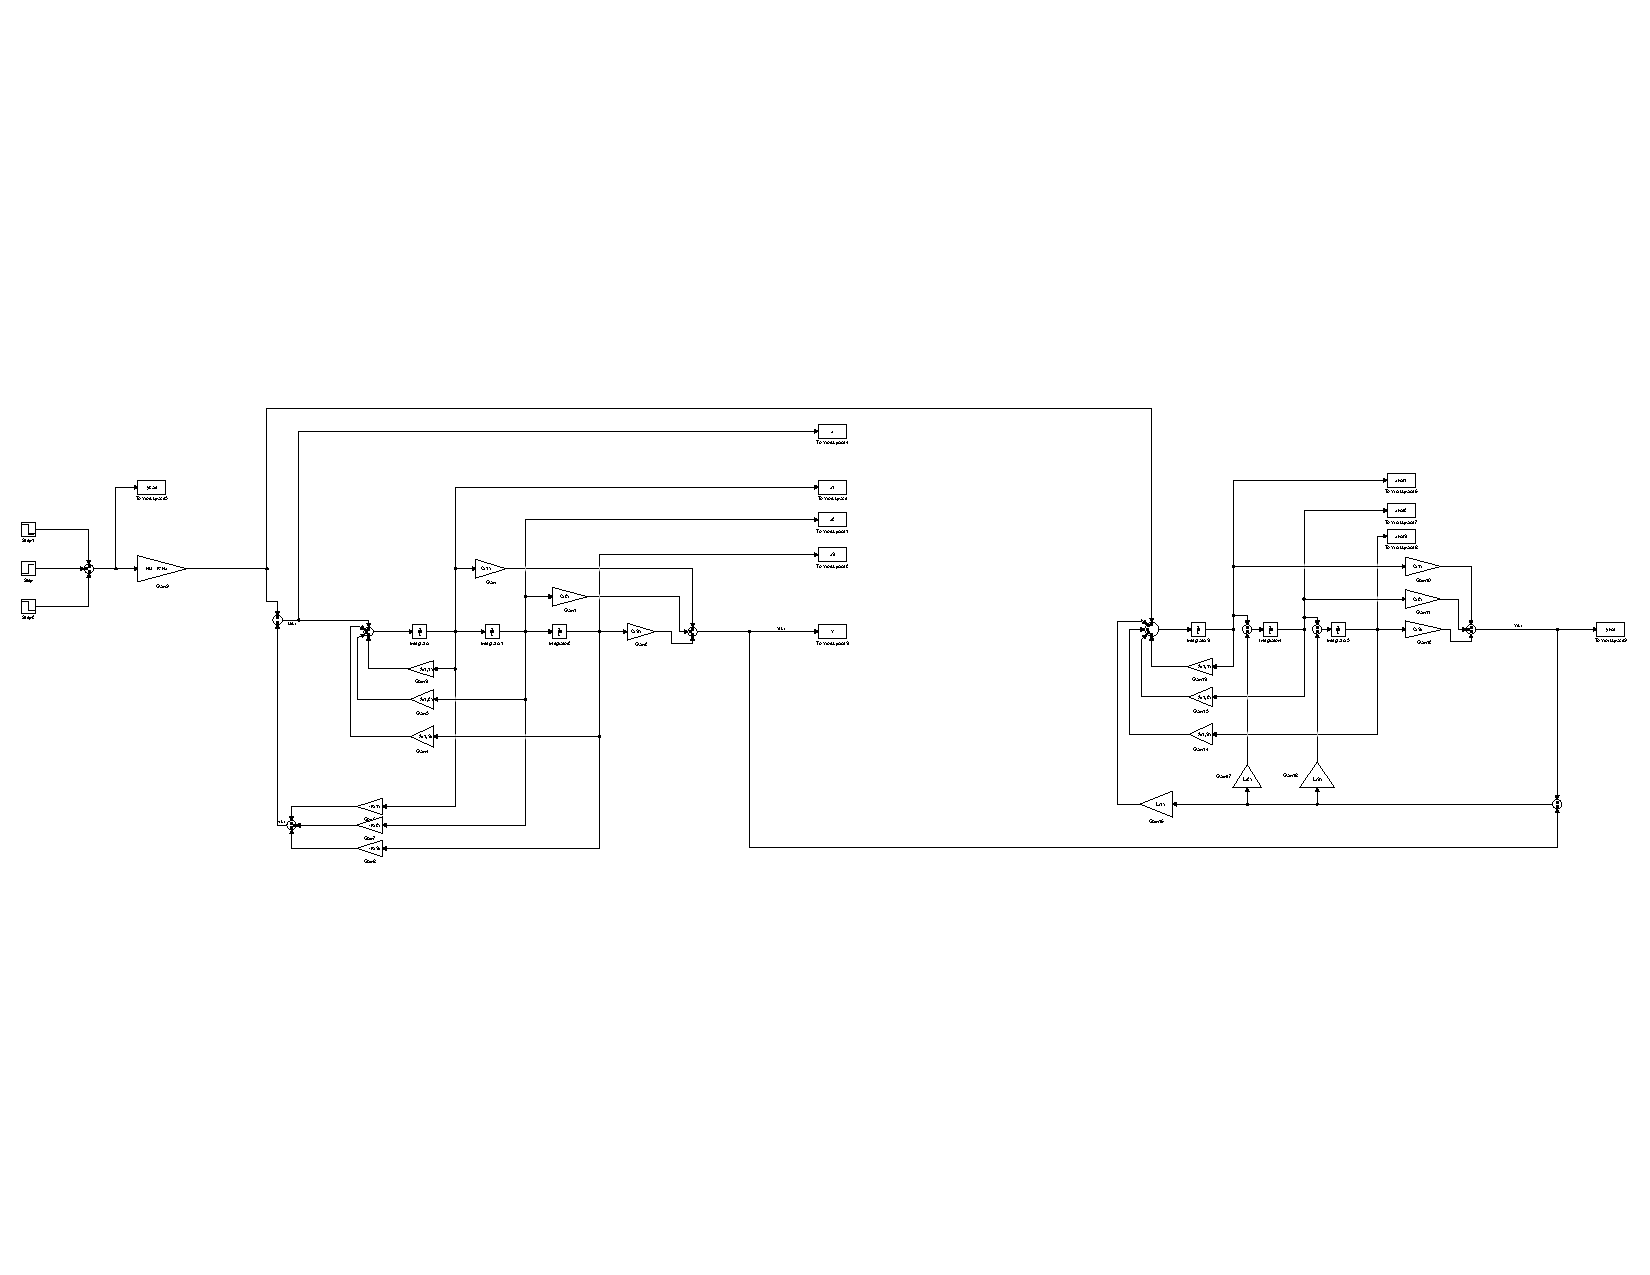
\includegraphics[width=0.9\linewidth]{z8sim}
\caption{Szczegółowa struktura obserwatora pełnego rzędu}
\label{fig:z8sim}
\end{figure}

Korzystając z funkcji \textit{acker()} wyznaczamy pierwiastki równania charakterystycznego:
\[|sI-(A-LC)| = 0\]

\section{Zadanie 9 - Symulacja obserwatora pełnego rzędu}
Pierwiastki obserwatora powinny mieć kilkukrotnie większy moduł, niż bieguny regulatora. Przetestowano regulator dla układu z biegunami regulacji $s_1 = s_2 = s_3 = -2$ (rys. \ref{fig:z8_-1}, \ref{fig:z8_-6}, \ref{fig:z8_-20}) oraz $s_1 = -1; s_2 = -2 + 0.1i; s_3 = -2 -0.1i$ (rys. \ref{fig:z8_2-1}, \ref{fig:z8_2-6}, \ref{fig:z8_2-20}).

\begin{figure}[H]
\centering
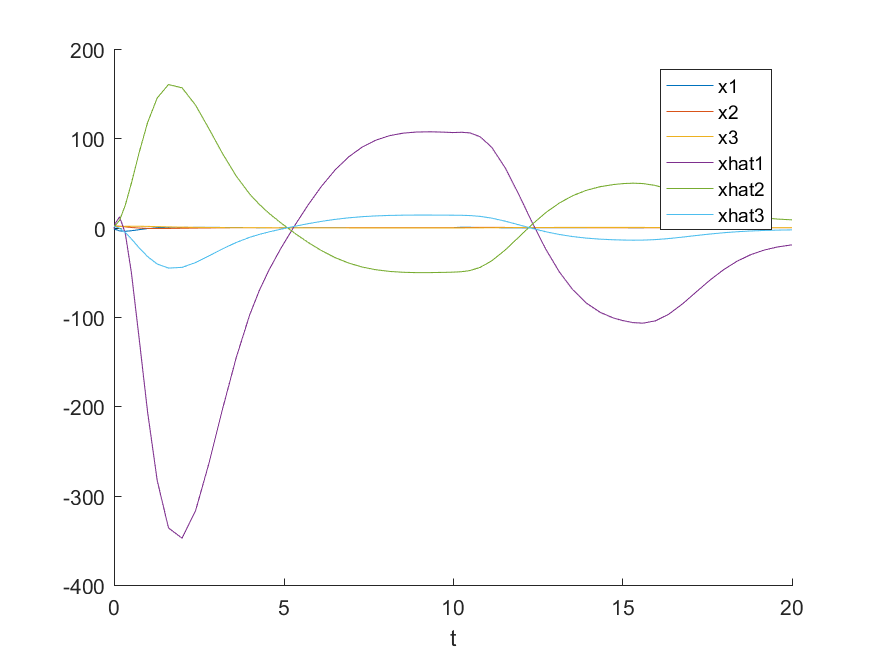
\includegraphics[width=0.9\linewidth]{z8_-1}
\caption{Wynik symulacji dla $s_1 = s_2 = s_3 = -2$ oraz $s_{o1}=s_{o2}=s_{o3} = -1$. Obserwator wolny. Obserwator nie nadąża.}
\label{fig:z8_-1}
\end{figure}

\begin{figure}[H]
\centering
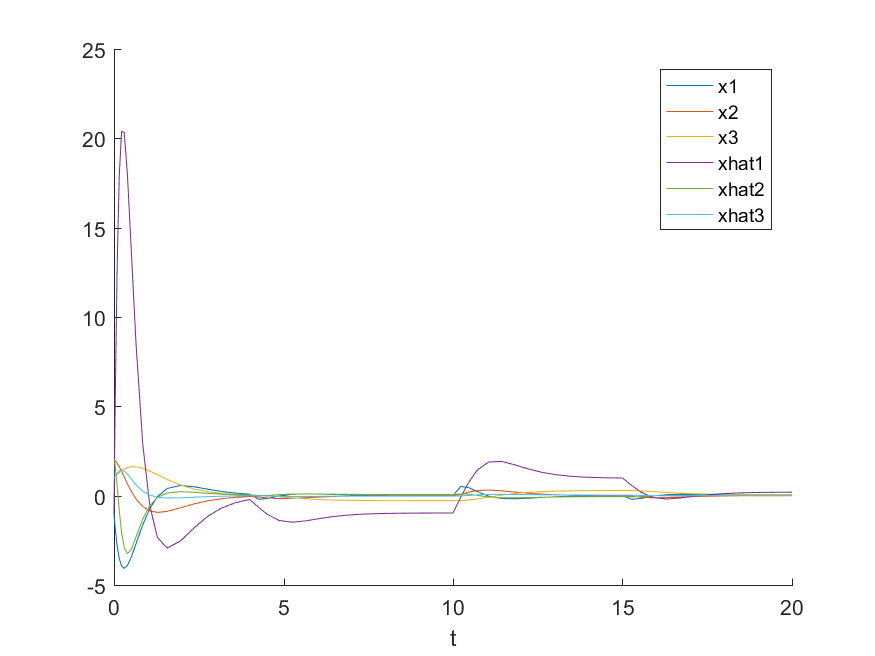
\includegraphics[width=0.9\linewidth]{z8_-6}
\caption{Wynik symulacji dla $s_1 = s_2 = s_3 = -2$ oraz $s_{o1}=s_{o2}=s_{o3} = -6$. Obserwator optymalny. Obserwator nadąża.}
\label{fig:z8_-6}
\end{figure}

\begin{figure}[H]
\centering
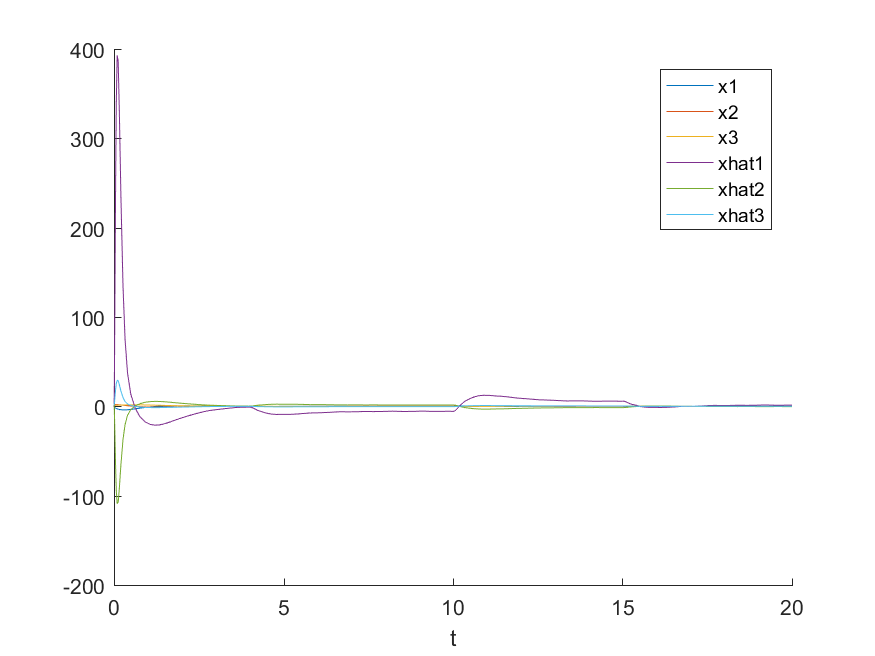
\includegraphics[width=0.9\linewidth]{z8_-20}
\caption{Wynik symulacji dla $s_1 = s_2 = s_3 = -2$ oraz $s_{o1}=s_{o2}=s_{o3} = -20$. Obserwator szybki. Obserwator nadąża. Początkowo duże zmiany zmiennych obserwatora i błędy estymacji.}
\label{fig:z8_-20}
\end{figure}

\begin{figure}[H]
\centering
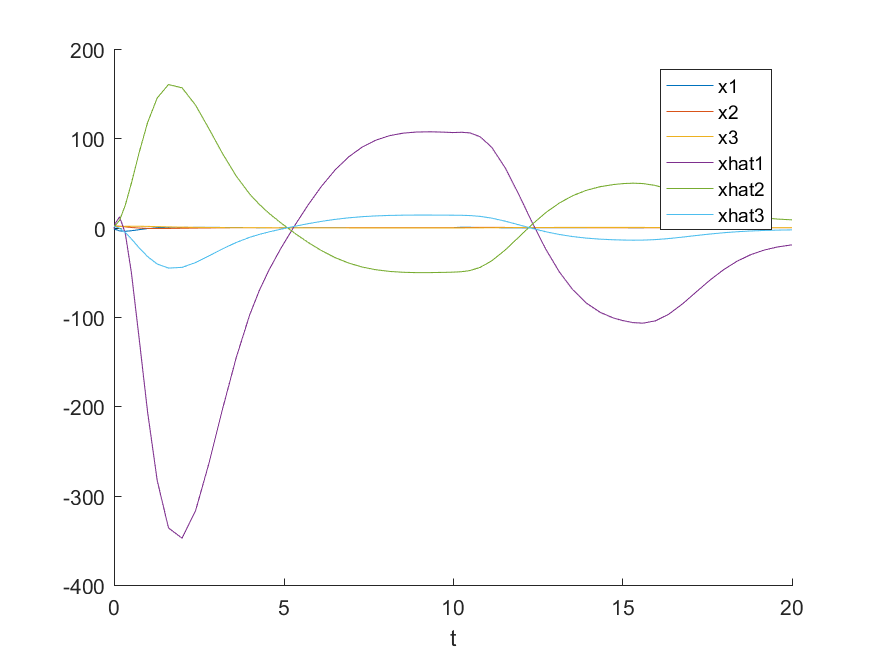
\includegraphics[width=0.9\linewidth]{z8_-1}
\caption{Wynik symulacji dla $s_1 = -1; s_2 = -2 + 0.1i; s_3 = -2 -0.1i$ oraz $s_{o1}=s_{o2}=s_{o3} = -1$. Obserwator wolny. Obserwator nie nadąża.}
\label{fig:z8_2-1}
\end{figure}

\begin{figure}[H]
\centering
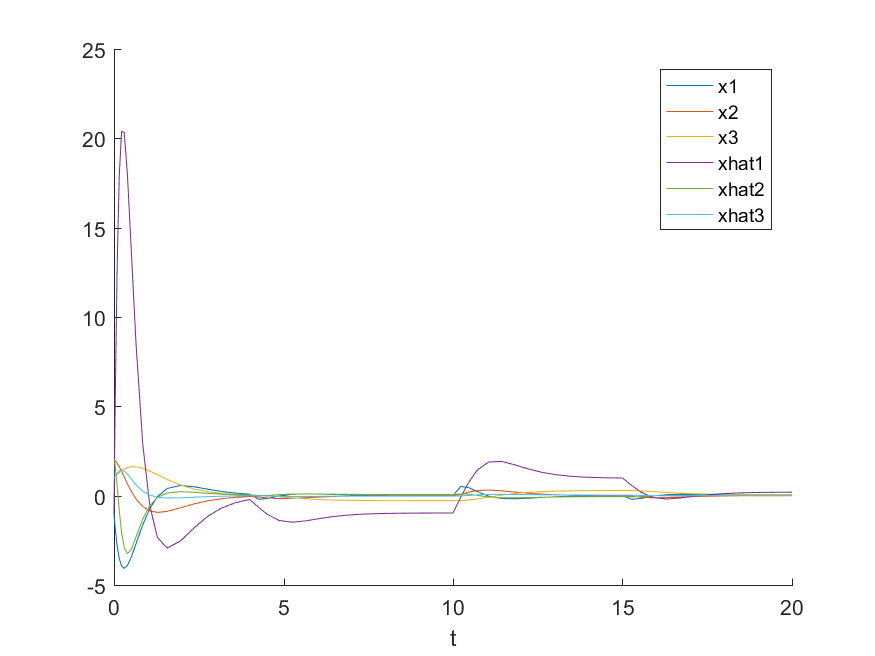
\includegraphics[width=0.9\linewidth]{z8_-6}
\caption{Wynik symulacji dla $s_1 = -1; s_2 = -2 + 0.1i; s_3 = -2 -0.1i$ oraz $s_{o1}=s_{o2}=s_{o3} = -6$. Obserwator optymalny. Obserwator nadąża.}
\label{fig:z8_2-6}
\end{figure}

\begin{figure}[H]
\centering
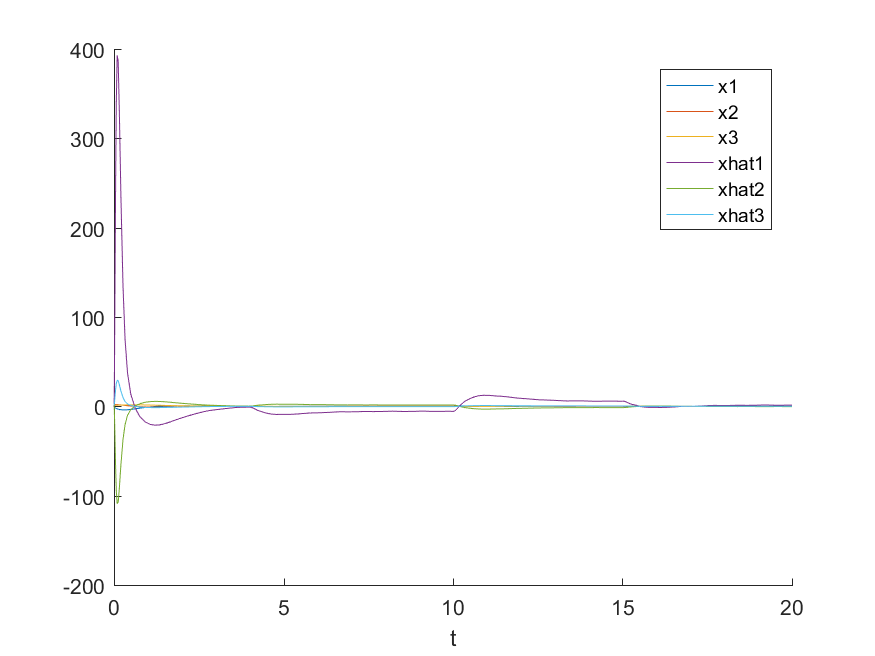
\includegraphics[width=0.9\linewidth]{z8_-20}
\caption{Wynik symulacji dla  $s_1 = -1; s_2 = -2 + 0.1i; s_3 = -2 -0.1i$ oraz $s_{o1}=s_{o2}=s_{o3} = -20$. Obserwator szybki. Obserwator nadąża. Początkowo duże zmiany zmiennych obserwatora i błędy estymacji.}
\label{fig:z8_2-20}
\end{figure}

\end{document}